%%%% PROCESAR con PdfLaTeX !!!!!


\documentclass[12pt]{book}
\usepackage{geometry}\geometry{top=2cm,bottom=2cm,left=3cm,right=3cm}
\usepackage{amssymb}
\usepackage{amsmath}
\usepackage{graphicx}
\usepackage{txfonts}




\begin{document}
\thispagestyle{empty}

\begin {center}

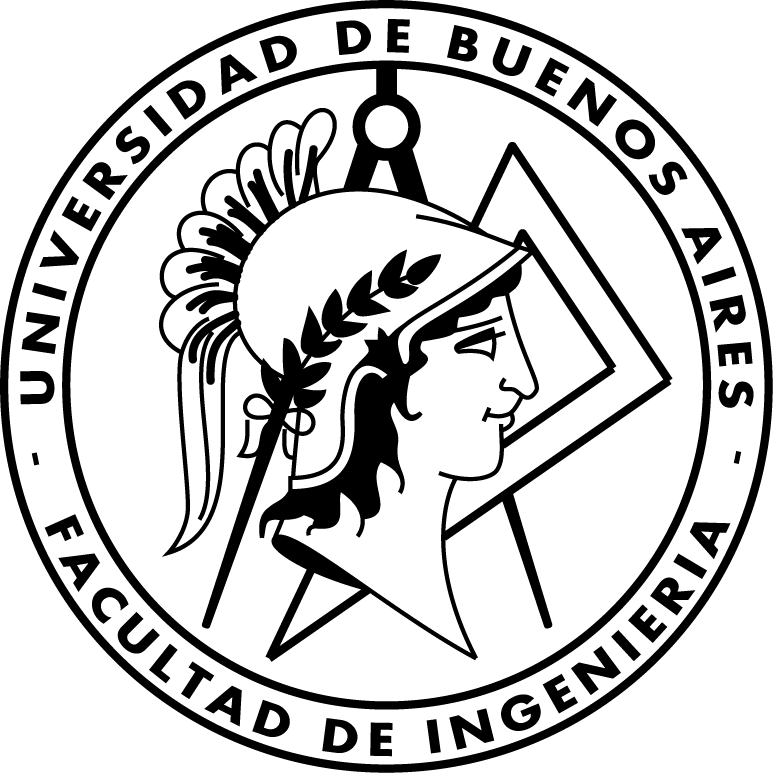
\includegraphics[scale=.4]{Logo-fiuba_big.png}

\medskip
UNIVERSIDAD DE BUENOS AIRES

Facultad de Ingenier\'ia

Departamento de Computaci\'on


\vspace{3cm}


\textbf{\large Introducci\'on a la complejidad Computacional}

\vspace{2cm}


Este es un modesto aporte para los alumnos de la f\'acultad de ingenier\'ia  de la UBA de las carreras de licenciatura en an\'alsis de sistemas e ingenier\'ia inform\'atica.
De ninguna man\'era pretende ser una gu\'ia de estudio, ni remplaza las clases presenciales, el material oficial de la catedra esta disponible en el web site de la m\'ateria.
\\
http://www.fi.uba.ar/node/36

\end {center}


\vspace{2.5cm}

\noindent Autor:\,	Isaac Edgar Camacho Ocampo
 
\noindent Carrera:\,	Licenciatura en An\'alisis de sistemas

\vspace{1cm}

\vspace{1cm}

\noindent Buenos Aires, 2019

\newpage


\tableofcontents

\tableofcontents
\chapter{Introducción}
En ciancias de la computacion existe una pregunat interesante, ¿cuanto nos cuesta un algoritmo? por ejemplo la busqueda binaria funciona mejor que una busqueda secuencial en base a que el arreglo estaria ordenado.
\\
\textbf{¿como podriamos medir el tiempo que consume un algoritmo?}
\\
Las respuestas pueden variar
\begin{itemize}
\item Tomamos un cronometro y medimos las ejecuciones del algoritmo.
\item Sumamos la cantidad de operaciones.
\item contamos la cantidad de codigo maquina que se genera despues de la compilacion.
\item y ¿como transmitimos los resaultados?
\end{itemize}

Si por ejemplo medimos la ejecucion un determinado algoritmo y nos resulta que tarda 3 ms, uno se puede preguntar, ¿Eso es r\'apido y lento?, si consideramos el paso del tiempo por ejemplo en 30 años seguramente eso seria lento, 
\textbf{¿Entonces como proceder?}

\section{El Algoritmo es inmutable}
Debemos percatarnos que el algoritmo es independiente del lenguaje de programaci\'on y de la maquina que lo ejecute, es decir en el papel es siempre el mismo!!!!.

Otra pregunta interesante es ¿ porque medir el tiempo ?, ya sea porque tenemos varios algoritmos y queremos ver cual tarda menos, siempre surge la necesidad de comparar dos algoritmos.
\\
El problema es encontrar un metodo de comparacion independiente de la implementacion.
las ideas de la introduccion no van a servir ya que dependen de las implementaciones.
\section{Usamos cotas - Notacion O}
\textbf{Notacion O} : esta notacion dice que la ecuacion de recurrencia que representa  al algoritmo 

\chapter{Fundamentos teóricos}
\section{Teoría clásica}
\subsection{Definición de variables}
\subsection{Pruebas y refutaciones}
\section{Hipótesis}
\chapter{Resultados}
\section{Simulación de resultados}
\subsection{Suposiciones}
\subsection{Modelos}
\section{Resultados preliminares}
\section{Resultados postprocesados}
\subsection{Valores atípicos}
\subsection{Correlaciones}
\chapter{Conclusiones}
\end{document}
